% Weak Scalability Design : Keep Pipeline of Ensembles to show barrier needed in S5 and S6
% Performance, generality with weak scaling (agnostic to kernel)
% Added functionality (do not speak about binding adaptivity to performance or generality)
% In use case: add in why TIES is challenging, and why adaptivity is challenging

% ---------------------------------------------------------------------------
\subsection{Experiment Setup}\label{ssec:exp_design}

We perform experiments to characterize the overheads of HTBAC, its runtime
system and the weak and strong scaling performance on NCSA Blue Waters and 
ORNL Titan. 


\begin{table*}
    \caption{Parameters of scalability experiments.}\label{tab:experiments}
    \centering
    \resizebox{\textwidth}{!}{
    \begin{tabular}{l            % Experiment ID
                    l            % CI
                    l            % protocol type
                    l            % number of protocols
                    l            % total cores
                    l            % executable
                    }
    %
    \toprule
    %
    \B{ID}                            &  % Experiment ID
    \B{Computing Infrastructure (CI)} &  % CI
    \B{Protocol(s)}                   &  % protocol type
    \B{No. Protocol(s)}                    &  % number of protocols
    \B{Total Cores}                    &  % total cores
    \B{Executable}                          \\ % executable
    %
    \midrule
    %
    \B{1}                             &  % Experiment ID
    Blue Waters                       &  % CI
    ESMACS                            &  % protocol type
    (2, 4, 8, 16)                     &  % number of protocols
    1600, 3200, 6400                  &  % total cores
    NAMD-MPI                               \\ % executable
    %
    \B{2}                             &  % Experiment ID
    Titan                          &  % CI
    ESMACS                          &  % protocol type
    (16, 64, 128)                    &  % number of protocols
    6400, 25600, 51200              &  % total cores
    NAMD (non-MPI)                 \\ % executable
    % 
    \B{3}                             &  % Experiment ID
    Blue Waters                       &  % CI
    TIES                              &  % protocol type
    (2, 4, 8)                         &  % number of protocols
    4160, 8320, 16640                 &  % total cores
    NAMD-MPI                              \\ % executable
    %
    \B{4}                             &  % Experiment ID
    Titan                          &  % CI
    TIES                          &  % protocol type
    (8, 32, 64)                    &  % number of protocols
    16640, 66560, 133120              &  % total cores
    NAMD (non-MPI)                 \\ % executable
    %
    \B{5}                             &  % Experiment ID
    Blue Waters                       &  % CI
    ESMACS + TIES                     &  % protocol type
    (2, 4, 8)                    &  % number of protocols
    5280, 10560, 21120              &  % total cores
    NAMD-MPI                              \\ % executable
    %
    \B{6}                             &  % Experiment ID
    Blue Waters                          &  % CI
    TIES                          &  % protocol type
    (8, 8, 8)                    &  % number of protocols
    16640, 8320, 4160              &  % total cores
    NAMD-MPI                              \\ % executable
    %
    \B{7}                             &  % Experiment ID
    Blue Waters                          &  % CI
    ESMACS                          &  % protocol type
    (16, 16, 16)                    &  % number of protocols
    6400, 3200, 1600              &  % total cores
    NAMD-MPI                              \\ % executable
    %
    \bottomrule
    %
    \end{tabular}
    }
\up{}
\end{table*}


We show homogeneous and heterogeneous weak scalability of the protocols by
growing the number of protocol instances while adhering to the required
number of pipelines. By design of each protocol, an increase in the number of
instances simply means an increase in the number of pipelines. The first weak
scalability experiment demonstrates the behavior of HTBAC, EnTK and RP using
the multiple instances of the ESMACS protocols on NCSA Blue Waters. The
second experiment shows weak scaling performance of ESMACS at higher scales,
using ORNL Titan.


The third and fourth experiments repeats the same design as experiments 1 and
2 yet demonstrate the performance of TIES. The fifth experiment demonstrates
concurrent execution of TIES and ESMACS in the same run. By design of weak
scaling, the ratio between the number of pipelines and cores are kept
constant. As the number of cores (measure of resource) changes by a factor of
2, we introduce twice as many protocol instances. As designed, the weak
scaling property provides insight into the size of the workload that can be
investigated in a given amount of time.

In addition, we demonstrate individual strong scaling performance of ESMACS
and TIES on Blue Waters in experiments 6 and 7, respectively. We fix the
number of protocols and vary the amount of resources in order to produce
generations of execution.

All Blue Waters experiments were performed from a persistent virtual machine,
as Blue Waters does not permit executing applications directly on the login
node. The ORNL Titan experiments had to be performed from an ORNL login node.
We used HTBAC version 0.1, EnTK version 0.6, and RP version 0.47. The MD
engine used is NAMD-MPI on Blue Waters. On Titan the MD engine is non-MPI
multi-core NAMD compiled with CUDA for ESMACS, while for TIES we compiled our
own internal non-CUDA multi-core OpenMP version as NAMD does not support
alchemical perturbations execution on GPU.

We perform all Blue Waters experiments using the APRUN launch method, which
has an upper limit of avg 436 concurrent task execution. In order to continue
execution on higher scales, we perform higher scales on ORNL Titan, using the
ORTE launch method. The difference in platforms produces overheads that can
be captured by RTS and are demonstrated in the figures as "APRUN overhead"
and "ORTE overhead".

For tasks pertaining to $S1$ - $S4$, while the analysis stage, $S5$ use
AmberTools. For both adaptive and nonadaptive experiments, the minimization
tasks of $S1$ are assigned 1000 steps, while the equilibration tasks in $S2$
and $S3$ are assigned 5000 steps. In the nonadaptive experiments, the
production simulation tasks in $S4$ are assigned 50,000 steps. For the
adaptive experiments, each substage of $S4$ i.e. $S4.1$ - $S4.4$ is assigned
50,000 steps.

% HTBAC submits a resource request to EnTK, to which EnTK uses RP to acquire
% resources via a single pilot. Accordingly, we request the maximum number of
% cores required by the workload as the number of cores in a pilot.

For weak scaling performance of TIES, we use between 4160 and 33280 cores as
indicated in Figure~\ref{fig:weak_scaling_TIES} because the NAMD executable
used in all tasks from $S1$-$S4$ require at least 32 cores per task. From our
own scalability performance measurements of NAMD on Blue Waters, we observe
the ideal cores per task to be 16, however Blue Waters does not permit
running multiple MPI applications on the same node, hence each NAMD task
requires a full node to maintain concurrency.

For strong scaling performance, we fix the number of protocol instances to 8
instances while varying the amount of resources as demonstrated in
Figure~\ref{fig:strong_scaling_TIES}.

For the TIES protocol, each pipeline consists of six stages. Each of the
simulation stages contains a task for every unique ($\lambda$, replica)
combination. In the non-adaptive workflow scenario, the first 11 $\lambda$
windows consist of the following values: $L$ is a vector with
\begin{flalign}
L &= \{ x_i: x_i\in[0,1]\; and\; x_{i+1} = x_i + \delta \}, where\ \delta\ is\ 0.1.
%&$$L=\{ x_i: x_i\in[0,1]\; and\; x_{i+1} = x_i + \delta \}$$%, where $\delta$ is $0.1$.
\end{flalign}

We append two additional values on both ends of $L$, completing 13 $\lambda$
windows. Each $\lambda$ window consists of five replicas. Therefore there are
a total of 65 tasks for every simulation stage. The production simulations
stage, $S4$ as described in figure~\ref{fig:pst} executes a 4 ns simulation
duration. The analysis stages of the protocol reduce the number of tasks. The
first analysis task consists of five tasks where each task performs an
aggregate analysis over all $\lambda$ windows for each replica. The second
analysis stage consists of one task that aggregates the previous results and
computes a single average across all replicas.

%----------------------------------------------------------------------------
\subsubsection{Scaling and Performance Characterization}

We first characterize the overheads of HTBAC and the runtime system. HTBAC
enables concurrent execution of multiple protocol instances. With each new
protocol instance generated for an application, the HTBAC overhead grows to
match the additional requirement of generating new protocols. The total time
to completion (TTC) can be expressed as following: $TTC = TTX + T_{O}$ where
 \(TTX\) measures the execution duration across all task, including file
 staging, MD kernel execution, pre- and post-executables, and $T_{O}$ the
 total overhead is given by the sum of the constituent overheads: $$T_{O} =
 T_{O}\textsuperscript{HTBAC} + T_{O}\textsuperscript{EnTK} +
 T_{O}\textsuperscript{RP}$$

% In order to understand the contribution of the various events in HTBAC,
% termed as HTBAC overhead, to

%----------------------------------------------------------------------------
% \subsubsection{Weak Scaling Experiments}

We investigated the weak scalability properties for the TIES protocol by
growing the number of protocol instances while adhering to the required
number of pipelines. By design of each protocol, an increase in the number of
instances simply means an increase in the number of pipelines. The first weak
scalability experiment demonstrates the behavior of HTBAC, EnTK and RP using
the multiple instances of the TIES protocol. By design of weak scaling, the
ratio between the number of pipelines and cores are kept constant. As the
number of cores (measure of resource) changes by a factor of 2, we introduce
twice as many protocol instances. As designed, the weak scaling property
provides insight into the size of the workload that can be investigated in a
given amount of time.

\begin{figure}
  \centering
    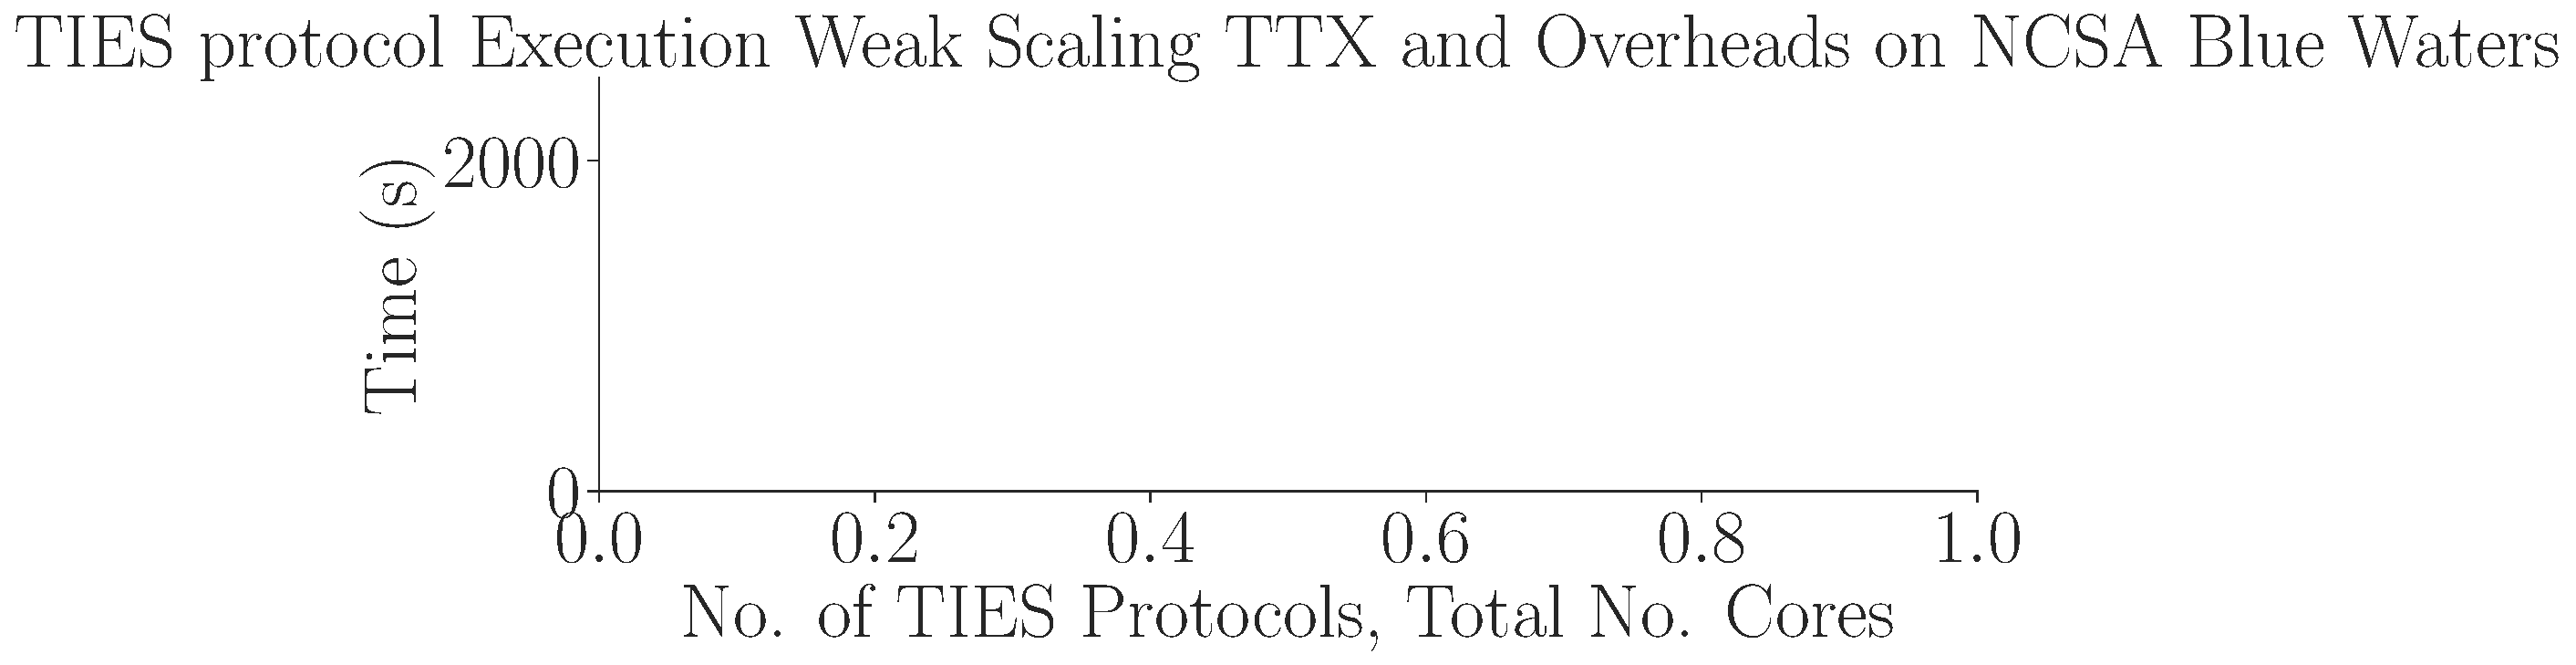
\includegraphics[width=\columnwidth]{figures/ties_ws_pseudo.pdf}
    \caption{Weak scaling properties of HTBAC. We investigate the weak
    scaling of HTBAC as the ratio of the number of protocol instances to
    resources is kept constant. Overheads of HTBAC (right), and runtime
    overhead (left) and \(TTX\) (left) for experimental configurations
    investigating the weak scaling of TIES. We ran X trials for each protocol
    instance configuration. Error bars in \(TTX\) in y-protocol runs are
    insignificant.}
\label{fig:weak_scaling_TIES}
\end{figure}

The second weak scalability experiment repeats the same experimental design
yet replaces the TIES protocols with TIES and ESMACS, respectively.

\begin{figure}
  \centering
    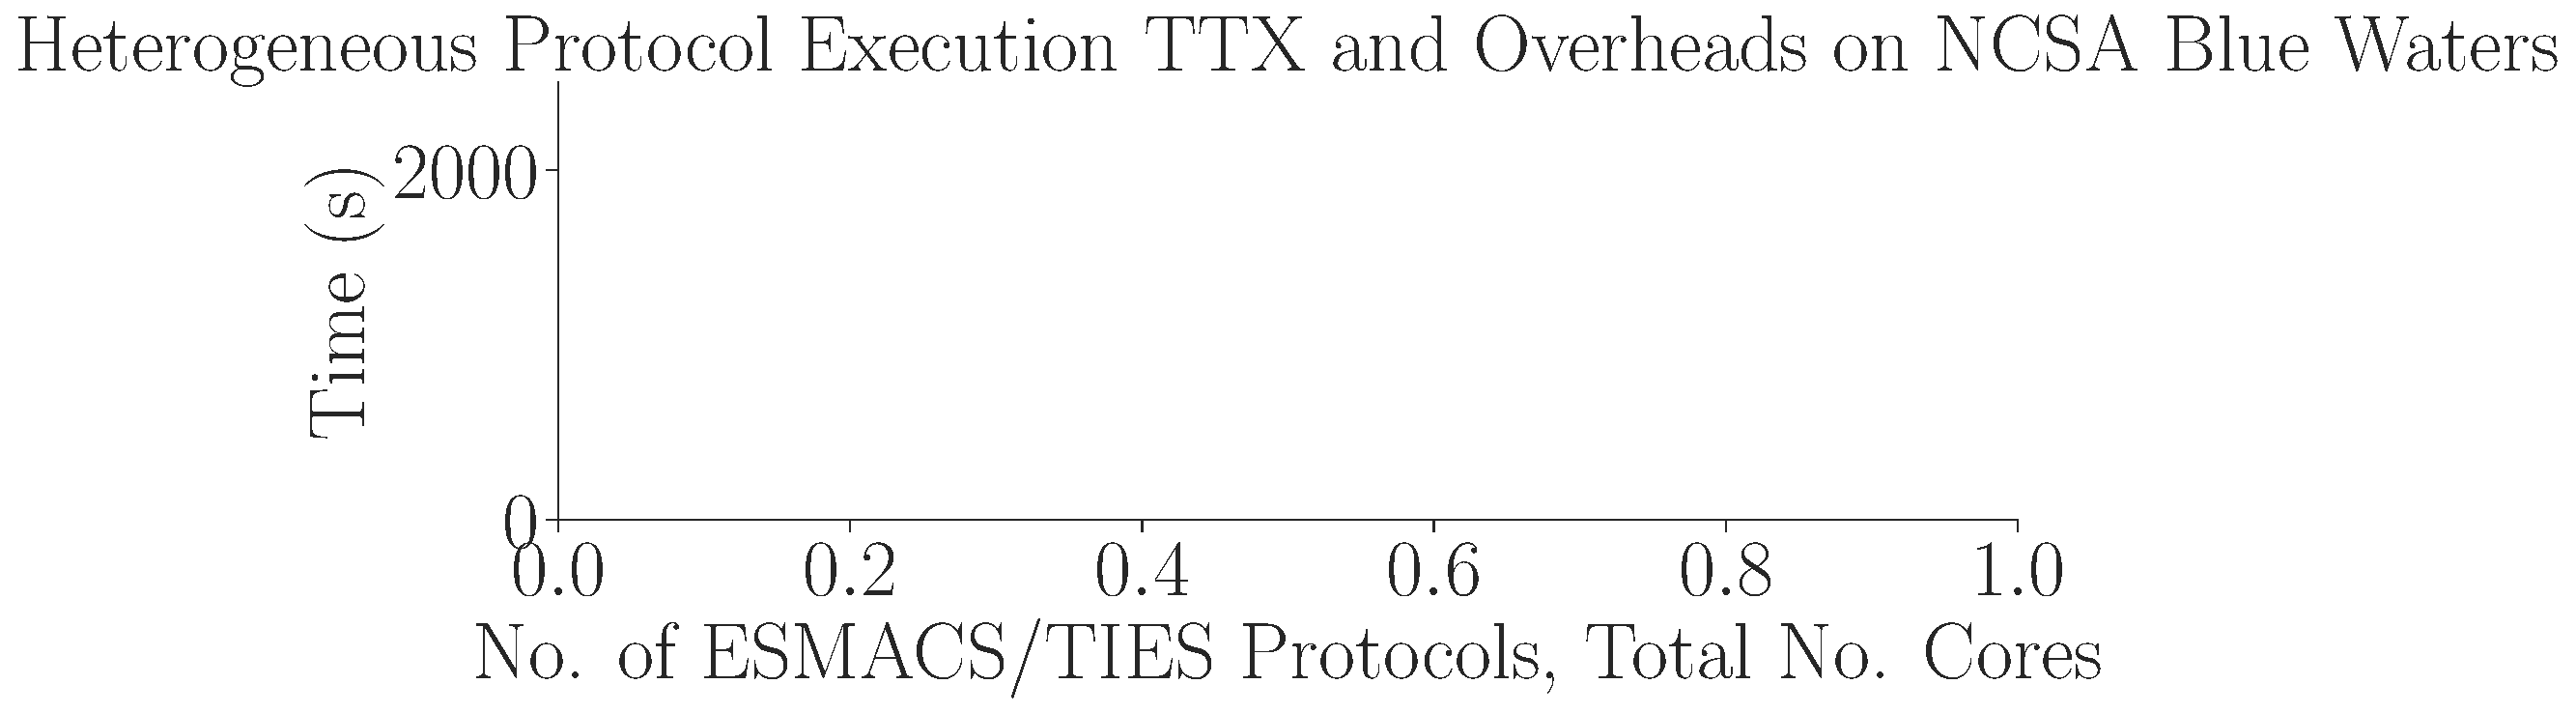
\includegraphics[width=\columnwidth]{figures/esmacs_ties_ws_pseudo.pdf}
    \caption{Weak scaling properties of HTBAC (right side). We investigate
    the weak scaling of HTBAC as the ratio of the number of ESMACS and TIES
    protocol instances to resources is kept constant. (Left) Overheads of
    HTBAC, and runtime overhead for experimental configurations. We ran X
    trials for each protocol instance configuration.}
\label{fig:weak_scaling_ESMACS_TIES}
\end{figure}


The HTBAC overhead shows a super linear increase as we grow the number of
protocol instances. However, the HTBAC overhead is a minimal contributor to
\(TTX\). The runtime overheads, mainly EnTK and RP, depend on the number of
tasks that need to be translated in-memory from a Python object to a compute
unit (CU) description. As such, it is expected to grow proportionally to the
number of tasks. EnTK submits CU descriptions to a MongoDB used by RP. RP
pilot pulls these descriptions from the same database.
% This pull operation occurs over a wide area networks, which introduces
% varying amounts of latency.
In addition, each stage constructed by EnTK maintains sequential barriers. RP
remains dormant until completion of the current tasks before staging the next
tasks \ref{fig:weak_scaling_ESMACS_TIES}.

% The impact of the synchronization barriers increases with the number of CUs
% as seen in the 16 protocol instances data point in

Furthermore, an additional overhead, driven by the aprun launch method,
increases as we approach a system limit on the number of permissible aprun
processes when scaling from 8 to 16 protocols, which translates to 520 and
1040 concurrent tasks, respectively. We account for the aprun failures in the
\(TTX\). Together, the EnTK-enabled synchronization barriers and aprun
overhead failures introduce delays in the scheduling of the CUs and results
in higher overheads. Lastly, we notice that each additional protocol instance
contributes to roughly 55 additional seconds in \(TTX\).

% ---------------------------------------------------------------------------
\subsubsection{Strong Scaling Experiments}

Next we repeat the same design of the weak scalability experiments but
examine performance of strong scaling when fixing the number of pipelines and
varying the resources. The comparison between weak and strong scalability
demonstrates the overhead introduced by load balancing and scheduling tasks
in multiple generations. As we scale the number of generation of concurrent
tasks executions, we half the resources allocated by the pilot.

Furthermore, as we scale the number of generations, the runtime overhead of
RP scales linearly. RP requires a proportional amount of time to schedule
tasks to the scale of execution. The main contributor to the increase in
overhead is derived by the time of resources inactivity while RP schedules
new tasks. As such, the overhead is expected to grow proportionally to the
number of concurrent tasks.

The RP overhead decomposes into events that capture the pilot and tasks
lifespan. The pilot duration contains the time to bootstrap and terminate the
pilot. The task overheads contain the executor's spawning of the task, folder
staging preparation, and operating system task spawning.

\begin{figure}
  \centering
    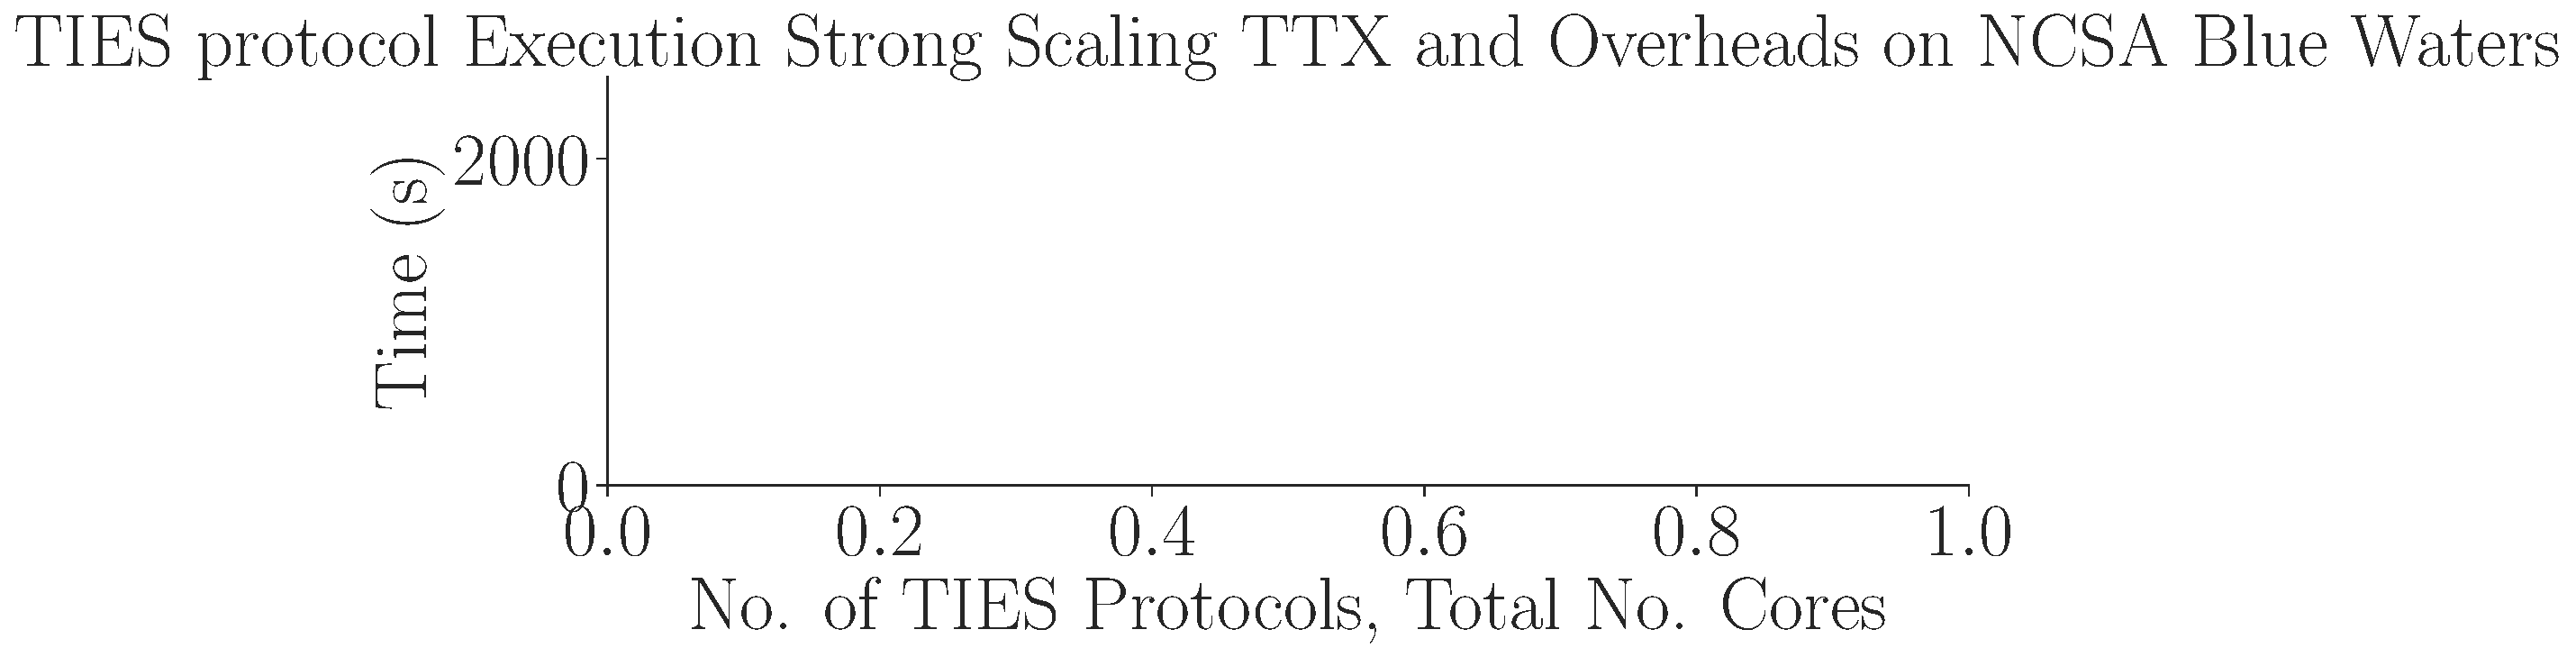
\includegraphics[width=\columnwidth]{figures/ties_ss_pseudo.pdf}
    \caption{Strong scaling properties of HTBAC using TIES protocols. We
    investigate the strong scaling of HTBAC with a fixed number of protocol
    instances while varying the amount resources. Overheads of HTBAC and
    runtime overhead (left) and \(TTX\) (right) for experimental
    configurations investigating the strong scaling of TIES.}
\label{fig:strong_scaling_TIES}
\end{figure}


(introduce experiment showing difference in overhead for EoP and PoE)


%----------------------------------------------------------------------------
\subsubsection{Validation Experiment}

HTBAC fully automates the process of calculating the binding affinity of
protein-ligand complexes from reading the input all the way to analyising the
final results. In order to validate the correctness of the results, we have
devised a set of experiments. These experiments are vital to gain confidence
in the algorithm and to prove that it is indeed calculating the correct
values.

The validation experiments were based on the original study of Wan et. al.
\cite{Wan2017brd4}. We selected a subset of the protein ligand systems that
were the subject of that study: they are the ligand transformations 3 to 1,
4, and 7. We then performed a full simulation on all 3 systems and calculated
the binding affinity (see Table~\ref{tab:exp2}) using HTBAC.

The results show that all three $\Delta \Delta$G values are within error bars
of the original study, reinforcing the fact that HTBAC has indeed correctly
implemented the complex workflow of TIES.

\begin{table}
  \centering
  \begin{tabular}{l@{\hskip 1in}r@{\hskip 0.2in}r@{\hskip 0.2in}r}
    \toprule
    System & HTBAC & Wan et. al & Experiment \\
    \midrule
    BRD4 \textbf{3 to 1} & \num{0.39 +- 0.10} &   \num{0.41 +- 0.04} &  \num{0.3 +- 0.09} \\
    BRD4 \textbf{3 to 4} & \num{0.02 +- 0.12} &   \num{0.01 +- 0.06} &  \num{0.0 +- 0.13} \\
    BRD4 \textbf{3 to 7} & \num{-0.88 +- 0.17} &  \num{-0.90 +- 0.08} & \num{-1.3 +- 0.11} \\
    \bottomrule
  \end{tabular}
  \caption{Comparison of the calculated binding free energies using HTBAC,
  from the original study by Wan et. al and experimental data. The two
  theoretical studies used the same protcol in principle. This experiment
  proved that HTBAC has indeed implemented TIES correctly, as the calculated
  values are either the same or within error bar of the original study. All
  values are in \textbf{kcal mol\textsuperscript{-1}}.}
  \label{tab:exp2}
\end{table}

%----------------------------------------------------------------------------
\subsubsection{Adaptive Experiments}

The TIES workflow can benefit from an adaptive execution environment to
improve the efficiency and accuracy of result. In \emph{adaptive experiments}
we implemented the adaptive quadrature algorithm specifically customized for
biosimulations.

In the adaptive workflow, over the course of a protocol instance we alter the
number of $\lambda$ windows being simulated. The position of new $\lambda$
windows depends on the estimated error of the integral measured between
adjacent windows. Increasing the number of $\lambda$ windows in regions of
rapid change will increase the accuracy of the overall integral to a greater
degree than an arbitrarily placed window. In order to adaptively add lambda
windows, we need access to the $\partial U/\partial\lambda$ values during
runtime. Therefore, we break down the single production simulation stage (S4)
from the nonadaptive workflow into multiple smaller stages, each running for
1 ns. Once each simulation is complete within a stage a decision is made
about whether more $\lambda$ windows are required, and if so where they
should be placed.

We start out the simulation with 5 replicas of \emph{3} equally spaced
$\lambda$ windows, and equilibrate them. Then we repeatedly execute shorter
production simulations followed by an analysis phase which determines where
to place new lambda windows. This procedure is repeated until convergence, at
which point all concurrent simulation are terminated. We define convergence
as the point in the production-analysis loop at which a desired error
threshold is reached.

The success of this algorithm is determined by the decision where additional
$\lambda$ windows should be introduced. In adaptive quadrature, this decision
is made by calculating an error estimate on the integral and comparing this
to a threshold value. Due to the stochastic nature of biosimulations, it is
non-trivial to determine this error, and as a proof of concept we simplified
this decision to replicate pre-calculated results. In future studies we plan
to replace this with a dynamic decision process.

Inter-node communication introduces a constraint on the number of new lambda
windows that can be added at each iteration. To reduce the overhead of
inter-node communication, simulations must run on an integer number of nodes.
This means that the number of new $\lambda$ windows (i.e. the number of
simulations) \emph{has} to be either doubled or left unchanged. If the number
of window is doubled the nodes per simulation can be halved automatically.
Our prototype algorithm loops through the current $\lambda$ window pairs
until this criterion is reached, forcefully adding more if needed.


% I don't think we need this equation here, it's too trivial.
% \begin{flalign}
% L &= \{ x_i: x_i\in[0,1]\; and\; x_{i+1} = x_i + \delta \}, where\ \delta\ is\ 0.5.
% %&$$L=\{ x_i: x_i\in[0,1]\; and\; x_{i+1} = x_i + \delta \}$$%, where $\delta$ is $0.1$.
% \end{flalign}

% For every $\lambda$ window we initialize with five replicas therefore yielding a
% total of 15 tasks. We run 15 tasks for stages $S1$ through $S4.1$. Between
% stages $S4.1$ and $S4.3$ the number of $\lambda$ windows doubles
% for every stage, which doubles the total number of tasks. The last production
% simulation stage, $S4.4$, runs for the remaining 2 ns durations.

We introduce only a single degree of freedom relative to baseline ``non-
adaptive" experiments, thus our experiments implement adaptive change in the
$\lambda$ windows sampled and not the timing of execution. HTBAC provides the
functional capability to adaptively determine the time at which the $\lambda$
windows are chosen. However in this paper, we do not investigate the impact
of such adaptivity, as the objective is to determine the feasibility of
adaptive execution and resulting scientific merit of adaptive decision
making.

% \begin{figure}
%   \centering
%    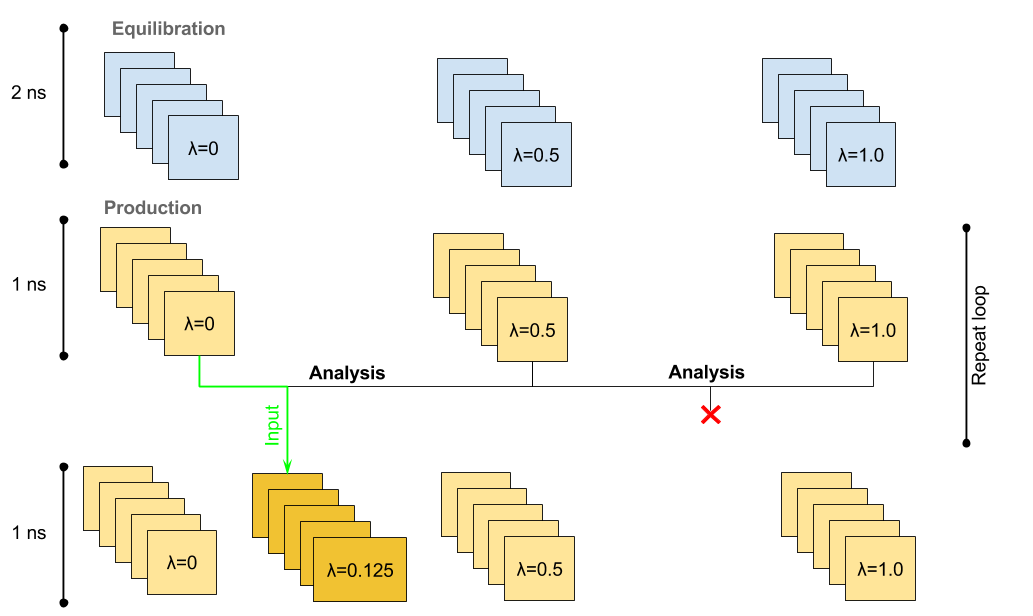
\includegraphics[width=\columnwidth]{figures/Adaptive_TIES_1.png}
%   \caption{Illustrating the adaptive workflow. After the 3 initial lambda 
%   windows are equilibrated, the first production stage starts. 
%   This is followed by analysis at every lambda interval, to decide whether 
%   to add a new window in the middle. The production-analysis is repeated 
%   for 4 production steps in our implementation, not shown here.}
% \label{fig:adaptive_TIES}
% \end{figure}

\begin{figure}
  \centering
    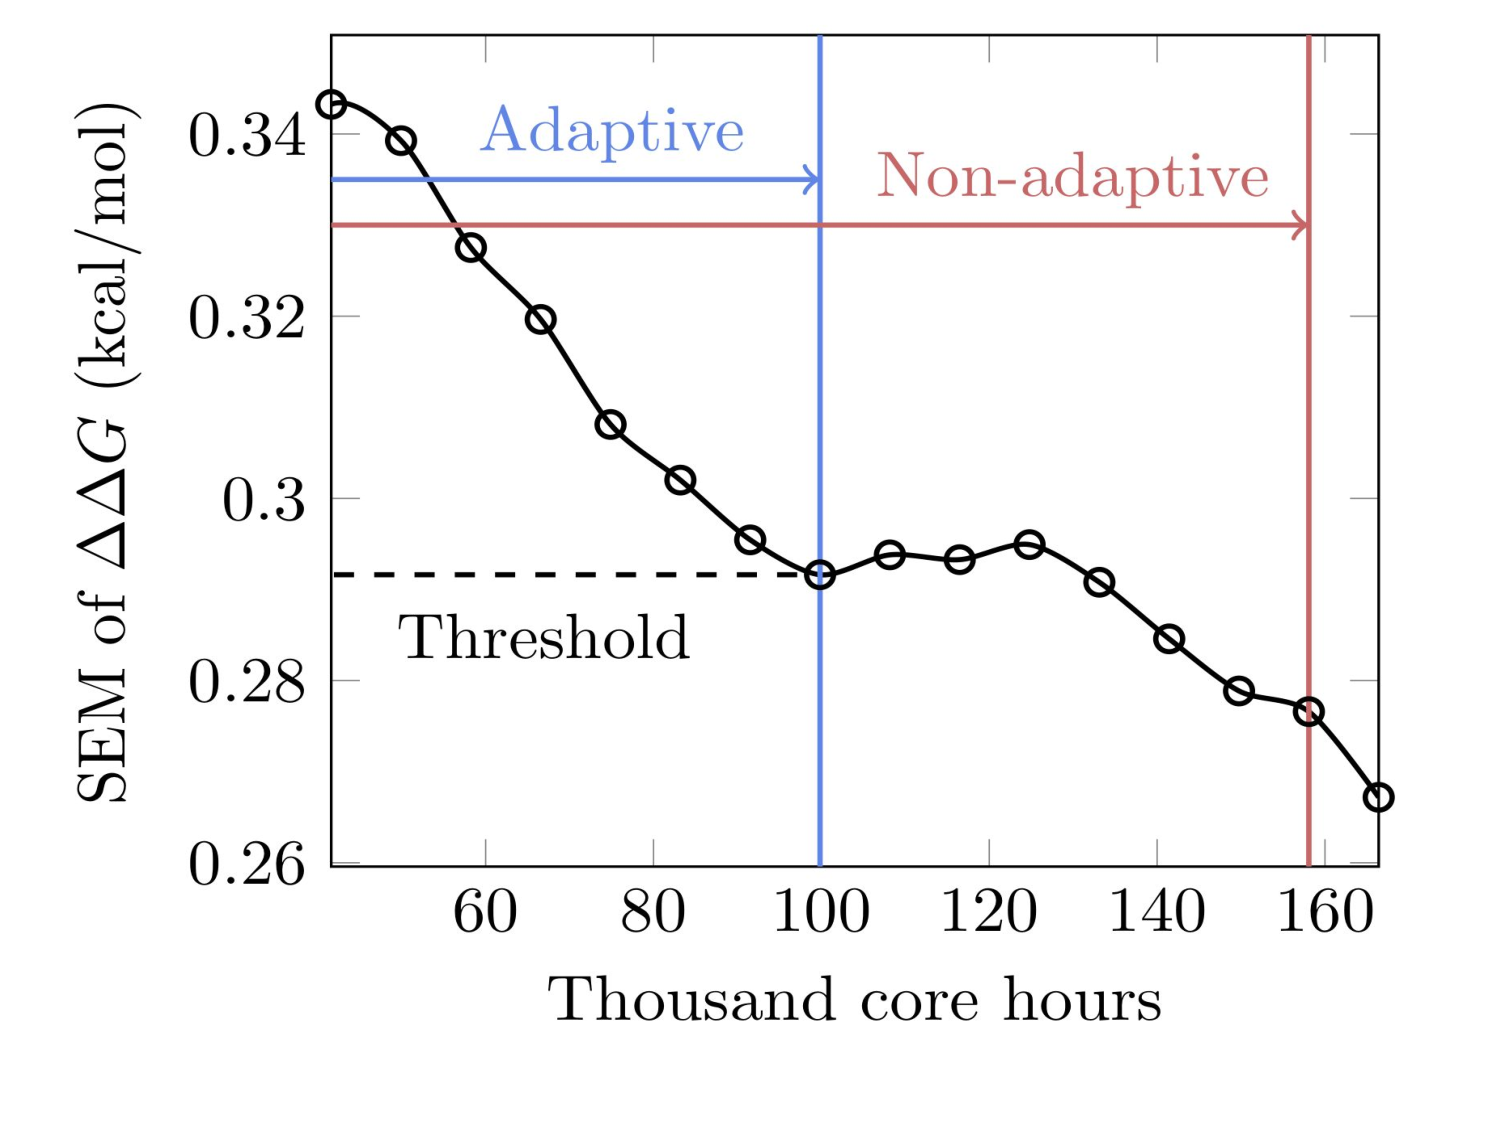
\includegraphics[width=\columnwidth]{figures/adaptive_vs_nonadaptive_pseudo.pdf}
    \caption{Illustrating the adaptive vs. non-adaptive workflow given the
    same number of core hours}
\label{fig:adaptive_vs_nonadaptive_TIES}
\end{figure}

% ---------------------------------------------------------------------------
\subsubsection{Adaptive Quadrature Experiments Results}

One way to visualize the adaptivity in this experiment is to plot the
function and integral approximations at every iteration.
Figure~\ref{fig:adapt} shows how the value of $\Delta$G (i.e. the integral of
the function) for test system \textbf{3 to 7} improves as the algorithm
places more lambda windows. It is imporant to note, that the new points are
decided {\it a priori} for reasons discussed above but this is opaque to the
algorithm. This is a proof that we have the adaptive capabilities and which
pave the way for more advanced biosimulation algorithms.

\begin{figure}
  \centering
\begin{tikzpicture}
\begin{axis}[
  xlabel=$\lambda$,
  ylabel=$\frac{dU}{d\lambda}$,
  xmin=0,
  xmax=1,
  legend pos=north west,
  grid=both,
  ]
  \addplot+[name path=alch_1, mark size=1pt, mark=*, color=blue] table [x=lambda, y=p1v]{alch_1.csv};
  \addlegendentry{Iteration 1: Initial};

  \addplot+[name path=alch_2, mark size=1pt, mark=*, color=red] table [x=lambda, y=p1v]{alch_2.csv};
  \addlegendentry{Iteration 2: Increase};

  \addplot+[name path=alch_3, mark size=1pt, mark=*, color=brown] table [x=lambda, y=p1v]{alch_3.csv};
  \addlegendentry{Iteration 3: Optimized};

  \addplot+[name path=alch_4, mark size=1pt, mark=*, color=black] table [x=lambda, y=p1v]{alch_4.csv};
  \addlegendentry{Iteration 4: Sampling};

  \addplot[name path=line, draw=none] {0};

  \addplot fill between[
    of = alch_1 and line,
    split,
    every even segment/.style = {pattern color=blue!50, pattern=vertical lines},
    every odd segment/.style = {pattern color=blue!50, pattern=vertical lines},
    soft clip={domain=0:1},
  ];

  \addplot fill between[
    of = alch_2 and line,
    split,
    every even segment/.style = {pattern color=red!50, pattern=horizontal lines},
    every odd segment/.style = {pattern color=red!50, pattern=horizontal lines},
    soft clip={domain=0:1},
  ];

  \addplot fill between[
    of = alch_3 and line,
    split,
    every even segment/.style = {pattern color=brown!50, pattern=north east lines},
    every odd segment/.style = {pattern color=brown!50, pattern=north east lines},
    soft clip={domain=0:1},
  ];

\end{axis}
\end{tikzpicture}
\caption{Approximating the intergral under the curve, hence calculating
$\Delta$G. The adaptive algorithm reevaluates the efficiency of the lambda
window mesh after every \SI{1}{\nano\second} and makes a decision whether to
place more lambda windows inside certain ranges. As we iterate every 1 ns,
the integral approximation becomes more accurate.}
\label{fig:adapt}
\end{figure}
